% Options for packages loaded elsewhere
\PassOptionsToPackage{unicode}{hyperref}
\PassOptionsToPackage{hyphens}{url}
\documentclass[
  ignorenonframetext,
]{beamer}
\newif\ifbibliography
\usepackage{pgfpages}
\setbeamertemplate{caption}[numbered]
\setbeamertemplate{caption label separator}{: }
\setbeamercolor{caption name}{fg=normal text.fg}
\beamertemplatenavigationsymbolsempty
% remove section numbering
\setbeamertemplate{part page}{
  \centering
  \begin{beamercolorbox}[sep=16pt,center]{part title}
    \usebeamerfont{part title}\insertpart\par
  \end{beamercolorbox}
}
\setbeamertemplate{section page}{
  \centering
  \begin{beamercolorbox}[sep=12pt,center]{section title}
    \usebeamerfont{section title}\insertsection\par
  \end{beamercolorbox}
}
\setbeamertemplate{subsection page}{
  \centering
  \begin{beamercolorbox}[sep=8pt,center]{subsection title}
    \usebeamerfont{subsection title}\insertsubsection\par
  \end{beamercolorbox}
}
% Prevent slide breaks in the middle of a paragraph
\widowpenalties 1 10000
\raggedbottom
\AtBeginPart{
  \frame{\partpage}
}
\AtBeginSection{
  \ifbibliography
  \else
    \frame{\sectionpage}
  \fi
}
\AtBeginSubsection{
  \frame{\subsectionpage}
}
\usepackage{iftex}
\ifPDFTeX
  \usepackage[T1]{fontenc}
  \usepackage[utf8]{inputenc}
  \usepackage{textcomp} % provide euro and other symbols
\else % if luatex or xetex
  \usepackage{unicode-math} % this also loads fontspec
  \defaultfontfeatures{Scale=MatchLowercase}
  \defaultfontfeatures[\rmfamily]{Ligatures=TeX,Scale=1}
\fi
\usepackage{lmodern}
\usetheme[]{Madrid}
\usecolortheme[]{dolphin}
\ifPDFTeX\else
  % xetex/luatex font selection
\fi
% Use upquote if available, for straight quotes in verbatim environments
\IfFileExists{upquote.sty}{\usepackage{upquote}}{}
\IfFileExists{microtype.sty}{% use microtype if available
  \usepackage[]{microtype}
  \UseMicrotypeSet[protrusion]{basicmath} % disable protrusion for tt fonts
}{}
\makeatletter
\@ifundefined{KOMAClassName}{% if non-KOMA class
  \IfFileExists{parskip.sty}{%
    \usepackage{parskip}
  }{% else
    \setlength{\parindent}{0pt}
    \setlength{\parskip}{6pt plus 2pt minus 1pt}}
}{% if KOMA class
  \KOMAoptions{parskip=half}}
\makeatother
\usepackage{graphicx}
\makeatletter
\newsavebox\pandoc@box
\newcommand*\pandocbounded[1]{% scales image to fit in text height/width
  \sbox\pandoc@box{#1}%
  \Gscale@div\@tempa{\textheight}{\dimexpr\ht\pandoc@box+\dp\pandoc@box\relax}%
  \Gscale@div\@tempb{\linewidth}{\wd\pandoc@box}%
  \ifdim\@tempb\p@<\@tempa\p@\let\@tempa\@tempb\fi% select the smaller of both
  \ifdim\@tempa\p@<\p@\scalebox{\@tempa}{\usebox\pandoc@box}%
  \else\usebox{\pandoc@box}%
  \fi%
}
% Set default figure placement to htbp
\def\fps@figure{htbp}
\makeatother
\setlength{\emergencystretch}{3em} % prevent overfull lines
\providecommand{\tightlist}{%
  \setlength{\itemsep}{0pt}\setlength{\parskip}{0pt}}
\usepackage{bookmark}
\IfFileExists{xurl.sty}{\usepackage{xurl}}{} % add URL line breaks if available
\urlstyle{same}
\hypersetup{
  pdftitle={Module 3: Statistical inference (II)},
  pdfauthor={Benjamin Smith},
  hidelinks,
  pdfcreator={LaTeX via pandoc}}

\title{\texorpdfstring{Module 3: Statistical inference
(II)}{Module 3: Statistical inference (II)}}
\author{\texorpdfstring{Benjamin Smith}{Benjamin Smith}}
\date{07/13/2026}

\begin{document}
\frame{\titlepage}

\begin{frame}{Outline}
\protect\phantomsection\label{outline}
This module we will review

\begin{itemize}
\tightlist
\item
  Basics of hypothesis testing
\item
  Central Limit Theorem
\item
  The Wald test
\item
  The score test
\item
  The likelihood ratio test
\end{itemize}
\end{frame}

\begin{frame}{Hypothesis testing}
\protect\phantomsection\label{hypothesis-testing}
\begin{block}{Definition (Hypothesis testing)}
\protect\phantomsection\label{definition-hypothesis-testing}
Suppose that we partition the parameter space \(\Theta\) into two
disjoint sets \(\Theta_{0}\) and \(\Theta_{1}\) and that we wish to test
\[
H_{0}: \theta \in \Theta_{0} \quad \text { versus } \quad H_{1}: \theta \in \Theta_{1}
\]
\end{block}

We call \(H_{0}\) the null hypothesis and \(H_{1}\) the alternative
hypothesis.
\end{frame}

\begin{frame}{Rejection region}
\protect\phantomsection\label{rejection-region}
Let \(X\) be a random variable and let \(\mathcal{X}\) be the range of
\(X\). Rejection region is a subset of outcomes \(R \in \mathcal{X}\)

\[
\begin{aligned}
&X \in R \quad \Longrightarrow \quad \text { reject } H_{0} \\
&X \notin R \quad \Longrightarrow \quad \text { retain }\left(\text { do not reject) } H_{0}\right.
\end{aligned}
\]

Usually, the rejection region is \[
R=\{x: T(x)>c\}
\] where \(T\) is a test statistic and \(c\) is a critical value.
\end{frame}

\begin{frame}{Type I error and type II error}
\protect\phantomsection\label{type-i-error-and-type-ii-error}
\begin{itemize}
\item
  Type I error, also known as a ``false positive'': the error of
  rejecting a null hypothesis when it is actually true.
  \(P(X\in R|H_0)\).
\item
  Type II error, also known as a ``false negative'': the error of not
  rejecting a null hypothesis when the alternative hypothesis is the
  true state of nature. \(P(X\notin R|H_0)\).
\end{itemize}
\end{frame}

\begin{frame}{Power function}
\protect\phantomsection\label{power-function}
\begin{block}{Definition (Power function)}
\protect\phantomsection\label{definition-power-function}
In a test of hypothesis about a parameter \(\theta\), let the null
hypothesis be \(H_0:\theta = \theta_0\). The power function
\(\beta(\theta)\) is a function that gives, for any \(\theta\), the
probability of rejecting the null hypothesis when the true parameter is
equal to \(\theta\).

\[
P(X\in R |\theta \text{ is the true parameter})
\]
\end{block}

Note that the power function depends on the null hypothesis: if we
change \(\theta_0\), also the power function changes.
\end{frame}

\begin{frame}{Size of a test}
\protect\phantomsection\label{size-of-a-test}
\begin{block}{Definition (The size of a test)}
\protect\phantomsection\label{definition-the-size-of-a-test}
The size of a test is defined to be \[
\alpha=\sup _{\theta \in \Theta_{0}} \beta(\theta) .
\] A test is said to have level \(\alpha\) if its size is less than or
equal to \(\alpha\).
\end{block}

Intuitively, we consider all the cases in which the null is true
(\(\theta \in \Theta_{0}\)). For each case, we compute the probability
of (incorrect) rejection. The size is equal to the largest value we find
(worst-case scenario).
\end{frame}

\begin{frame}{Exercise}
\protect\phantomsection\label{exercise}
Let \(X_{1}, \ldots, X_{n} \sim N(\mu, \sigma)\) where \(\sigma\) is
known. We want to test \(H_{0}: \mu \leq 0\) versus \(H_{1}: \mu>0\).
Hence, \(\Theta_{0}=(-\infty, 0]\) and \(\Theta_{1}=(0, \infty)\).

Consider the test: \[ \text{reject } H_{0} \text{ if } T>c \] where
\(T=\bar{X}\). The rejection region is \[
R=\left\{\left(x_{1}, \ldots, x_{n}\right): T\left(x_{1}, \ldots, x_{n}\right)>c\right\}
\]

What is the power function? What is the size of the test?
\end{frame}

\begin{frame}{Exercise (cont'd)}
\protect\phantomsection\label{exercise-contd}
Let \(Z\) denote a standard Normal random variable. The power function
is \[
\begin{aligned}
\beta(\mu) &=\mathbb{P}_{\mu}(\bar{X}>c) \\
&=\mathbb{P}_{\mu}\left(\frac{\sqrt{n}(\bar{X}-\mu)}{\sigma}>\frac{\sqrt{n}(c-\mu)}{\sigma}\right) \\
&=\mathbb{P}\left(Z>\frac{\sqrt{n}(c-\mu)}{\sigma}\right) \\
&=1-\Phi\left(\frac{\sqrt{n}(c-\mu)}{\sigma}\right)
\end{aligned}
\]
\end{frame}

\begin{frame}{Exercise (cont'd)}
\protect\phantomsection\label{exercise-contd-1}
\[
\text { size }=\sup _{\mu \leq 0} \beta(\mu)=\beta(0)=1-\Phi\left(\frac{\sqrt{n} c}{\sigma}\right)
\] For a size \(\alpha\) test, we set this equal to \(\alpha\) and solve
for \(c\) to get \[
c=\frac{\sigma \Phi^{-1}(1-\alpha)}{\sqrt{n}}
\] We reject when \(\bar{X}>\sigma \Phi^{-1}(1-\alpha) / \sqrt{n}\).
\end{frame}

\begin{frame}{Asymptotically normality}
\protect\phantomsection\label{asymptotically-normality}
\begin{block}{Definition}
\protect\phantomsection\label{definition}
We say that an estimator \(\hat{\theta}\) is asymptotically normal if:
\[
\frac{\hat{\theta}-\theta}{\sqrt{\operatorname{Var}(\hat{\theta})}} \stackrel{d}{\rightarrow} N(0,1)
\]
\end{block}

\begin{block}{Theorem}
\protect\phantomsection\label{theorem}
If an estimator is asymptotically normal and the scaled squared standard
error
\(\sqrt{n \widehat{\operatorname{Var}}(\hat{\theta})} \stackrel{P}{\rightarrow} \sqrt{n \operatorname{Var}(\hat{\theta})}\)
then \[
\frac{\hat{\theta}-\theta}{\sqrt{\widehat{\operatorname{Var}}(\hat{\theta})}} \stackrel{d}{\rightarrow} N(0,1)
\]
\end{block}
\end{frame}

\begin{frame}{Central Limit Thorem}
\protect\phantomsection\label{central-limit-thorem}
Let \(X_1, \ldots, X_n\) be a sequence of independent and identically
distributed (i.i.d.) random variables drawn from a distribution with
mean \(\mu\) and variance \(\sigma^2\). Then \[
\frac{\bar{X}_n-\mu}{\sqrt{\operatorname{Var}\left(\bar{X}_n\right)}}=\frac{\sqrt{n}\left(\bar{X}_n-\mu\right)}{\sigma} \stackrel{d}{\rightarrow} N(0,1) \text { as } n \rightarrow \infty
\] Proof: Omitted. By characteristic functions.
\end{frame}

\begin{frame}{Example}
\protect\phantomsection\label{example}
When
\(X_1, \ldots, X_n \stackrel{\text { i.i.d }}{\sim} N\left(\mu, \sigma^2\right)\),
then \(\bar{X}_n\) satisfies that
\(\frac{\bar{X}_n-\mu}{\sqrt{\operatorname{Var}\left(\bar{X}_n\right)}} \stackrel{d}{\rightarrow} N(0,1)\)
and \(\sqrt{n \operatorname{var}\left(\bar{X}_n\right)}=\)
\(\sqrt{n \frac{s^2}{n}}=s \stackrel{P}{\rightarrow} \sigma=\sqrt{n \operatorname{Var}\left(\bar{X}_n\right)}\).
Then we can use the theorem above to conclude that \[
\frac{\bar{X}_n-\mu}{\sqrt{\widehat{\operatorname{Var}}\left(\bar{X}_n\right)}} \stackrel{d}{\rightarrow} N(0,1).
\]
\end{frame}

\begin{frame}{The Wald test}
\protect\phantomsection\label{the-wald-test}
We are interested in testing the hypotheses in a parametric model: \[
H_{0}: \theta=\theta_{0} \quad \text { versus } H_{1}: \theta \neq \theta_{0} .
\] The Wald test most generally is based on an asymptotically normal
estimator, i.e.~we suppose that we have access to an estimator
\(\widehat{\theta}\) which under the null satisfies the property that:
\[
\widehat{\theta} \stackrel{d}{\rightarrow} N\left(\theta_0, \sigma_0^2\right)
\] where \(\sigma_0^2\) is the variance of the estimator under the null.
The canonical example is when \(\widehat{\theta}\) is taken to be the
MLE.
\end{frame}

\begin{frame}{The Wald statistic}
\protect\phantomsection\label{the-wald-statistic}
If the hypothesis involves only a single parameter restriction, then the
Wald statistic takes the following form: \[
W_n=\frac{\left(\hat{\theta}-\theta_0\right)^2}{\operatorname{var}(\hat{\theta})} ,
\] which under the null hypothesis follows an asymptotic
\(\chi^2_1\)-distribution with one degree of freedom.
\end{frame}

\begin{frame}{Example}
\protect\phantomsection\label{example-1}
Suppose we considered the problem of testing the parameter of a
Bernoulli, i.e.~we observe
\(X_1, \ldots, X_n \sim \operatorname{Ber}(p)\), and the null is that
\(p=p_0\). Defining \(\widehat{p}=\frac{1}{n} \sum_{i=1}^n X_i\). A Wald
test could be constructed based on the statistic: \[
T_n=\frac{(\widehat{p}-p_0)^2}{\frac{p_0\left(1-p_0\right)}{n}},
\] which has an asymptotic \(\chi^2_1\) distribution. An alternative
would be to use a slightly different estimated standard deviation,
i.e.~to define,

\[
T_n=\frac{(\widehat{p}-p_0)^2}{\frac{\widehat{p}\left(1-\widehat{p}\right)}{n}},
\] Observe that this alternative test statistic also has an
asymptotically \(\chi^2_1\) distribution under the null.
\end{frame}

\begin{frame}{The score test}
\protect\phantomsection\label{the-score-test}
Score test is based on the value of the score function \(U(\theta)\)
under the null hypothesis \(H_0\).

Reminder: \(U(\theta) = \ell^{\prime}(\theta)\).

The score test statistic

\[
S_n = \frac{U(\theta_0)^2}{\operatorname{var}[U(\theta_0)]},
\] which has an asymptotic distribution of \(\chi^2_1\) under the null.

Reminder: the variance of the score function is the Fisher information.
\end{frame}

\begin{frame}{The score test}
\protect\phantomsection\label{the-score-test-1}
Similary, we have

\[
\widehat{I}\left(\theta_{0}\right)=-\left.\frac{1}{n} \sum_{i=1}^{n} \frac{\partial^{2} \log f\left(x_{i} \mid \theta\right)}{\partial \theta^{2}}\right|_{\theta_{0}} \stackrel{\mathrm{P}}{\rightarrow} I\left(\theta_{0}\right)
\]

so that

\[
S_n = \frac{U(\theta_0)^2}{\widehat{I}\left(\theta_{0}\right)}
\]

also has an asymptotic distribution of \(\chi^2_1\) under the null.
\end{frame}

\begin{frame}{The likelihood ratio test}
\protect\phantomsection\label{the-likelihood-ratio-test}
Let \(\hat{\theta}_n\) be the MLE of \(\theta\).

\[
\Delta_{n}= \ell\left(\widehat{\theta}_{n}\right)-\ell\left(\theta_{0}\right) =\log \left(\frac{L(\hat{\theta}_n\mid\mathbf{x})}{L\left(\theta_{0} \mid \mathbf{x}\right)}\right) =\log \left(\frac{\sup _{\theta \in \Theta}(\theta \mid \mathbf{x})}{L\left(\theta_{0} \mid \mathbf{x}\right)}\right) \geq 0
\]

Under \(H_0\),

\[
2 \Delta_{n} \stackrel{\mathrm{D}}{\rightarrow} \chi_{1}^{2}
\]
\end{frame}

\begin{frame}{Uniformly most powerful test}
\protect\phantomsection\label{uniformly-most-powerful-test}
\begin{block}{Definition:}
\protect\phantomsection\label{definition-1}
In statistical hypothesis testing, a uniformly most powerful (UMP) test
is a hypothesis test which has the greatest power among all possible
tests of a given size \(\alpha\).
\end{block}

\begin{block}{Theorem (Neyman-Pearson lemma):}
\protect\phantomsection\label{theorem-neyman-pearson-lemma}
Let \(H_0\) and \(H_1\) be simple hypotheses. For a constant \(c>0\),
suppose that the likelihood ratio test which rejects \(H_0\) when
\(L(\mathbf{x})<c\) has significance level \(\alpha\). Then for any
other test of \(H_0\) with significance level at most \(\alpha\), its
power against \(H_1\) is at most the power of this likelihood ratio
test.
\end{block}
\end{frame}

\begin{frame}{The Wald test, score test, and likelihood ratio test}
\protect\phantomsection\label{the-wald-test-score-test-and-likelihood-ratio-test}
\begin{figure}
\centering
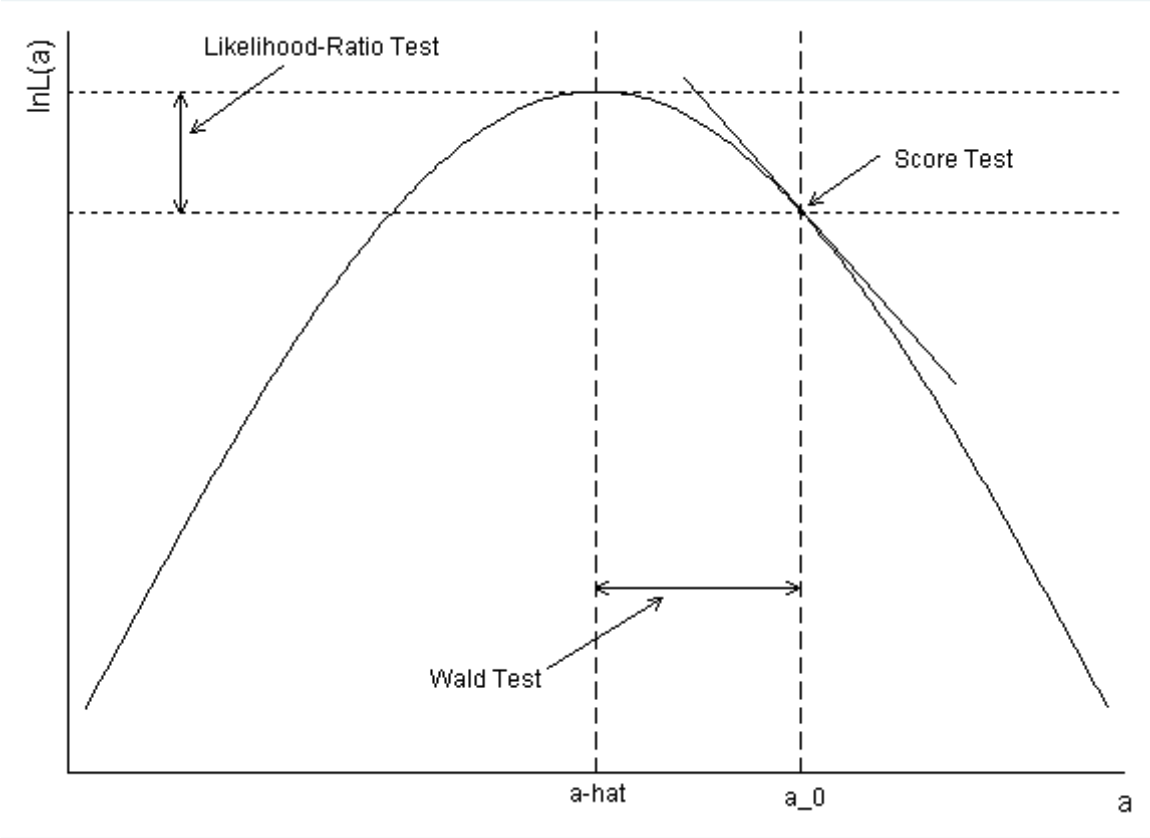
\includegraphics[width=\linewidth,height=0.8\textheight,keepaspectratio,alt={Fox, J. (1997) Applied regression analysis, linear models, and related methods. Thousand Oaks, CA: Sage Publications. P. 570.}]{comparison.png}
\caption{Fox, J. (1997) Applied regression analysis, linear models, and
related methods. Thousand Oaks, CA: Sage Publications. P. 570.}
\end{figure}
\end{frame}

\begin{frame}{Test equivalence}
\protect\phantomsection\label{test-equivalence}
We can show that (when there is no misspecification)

\begin{itemize}
\tightlist
\item
  The tests are asymptotically equivalent in the sense that under
  \(H_{0}\) they reach the same decision with probability 1 as
  \(n \rightarrow \infty\).
\item
  For a finite sample size \(n\), they have some relative advantages and
  disadvantages with respect to one another.
\end{itemize}
\end{frame}

\begin{frame}{Discussion}
\protect\phantomsection\label{discussion}
\[W_n=\frac{\left(\hat{\theta}-\theta_0\right)^2}{\operatorname{var}(\hat{\theta})} \stackrel{\mathrm{D}}{\rightarrow} \chi_{1}^{2}\]

\[S_n = \frac{U(\theta_0)^2}{\widehat{I}\left(\theta_{0}\right)} \stackrel{\mathrm{D}}{\rightarrow} \chi_{1}^{2}\]

\[2\Delta_{n}=2 \left\{ \ell\left(\widehat{\theta}_{n}\right)-\ell\left(\theta_{0}\right) \right\} \stackrel{\mathrm{D}}{\rightarrow} \chi_{1}^{2}\]

\begin{itemize}
\tightlist
\item
  It is easy to create one-sided Wald and score tests.
\item
  The score test does not require \(\widehat{\theta}_{n}\) whereas the
  other two tests do.
\item
  The Wald test is most easily interpretable and yields immediate
  confidence intervals.
\item
  The score test and LR test are invariant under reparametrization,
  whereas the Wald test is not.
\end{itemize}
\end{frame}

\begin{frame}{Resources}
\protect\phantomsection\label{resources}
This tutorial is based on

\begin{itemize}
\item
  ``All of statistics'' Chapter 10 by Larry A. Wasserman.
\item
  Arnaud Doucet's STA 461 Lecture notes
  {[}\href{https://www.cs.ubc.ca/~arnaud/stat461/lecture_stat461_WaldRaoLRtests_handouts_2008.pdf}{links}{]}.
\end{itemize}
\end{frame}

\end{document}
